\begin{frame}[fragile]{pause}\frametitle{Batch Normalization}
\begin{itemize}
\item Batch normalization (BN) is a technique for improving the performance of ANNs
\item It improves the stability of ANNs by adjusting and scaling the activations
\item BN makes your ANN more robust to the choice of hyperparameters (larger range of parameters that will work well)
\item It was introduced by Sergey Ioffe and Christian Szegedy in 2015 \footnote{\url{https://arxiv.org/pdf/1502.03167.pdf}}
\end{itemize}
\end{frame}
%-------------------------------------------------------------%

\begin{frame}[fragile]{pause}\frametitle{Batch Normalization}
\center{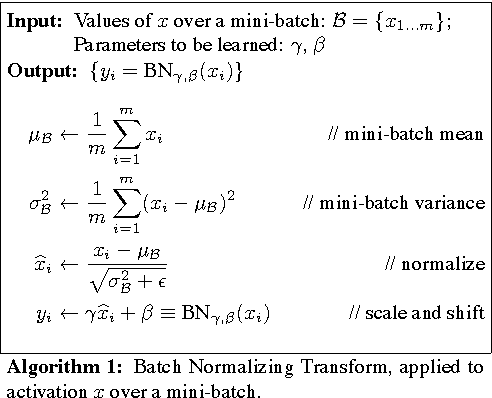
\includegraphics[width=0.9\textwidth]{batchnorm.pdf}}
\end{frame}
%-------------------------------------------------------------%

\begin{frame}[fragile]{pause}\frametitle{Batch Normalization}
\center{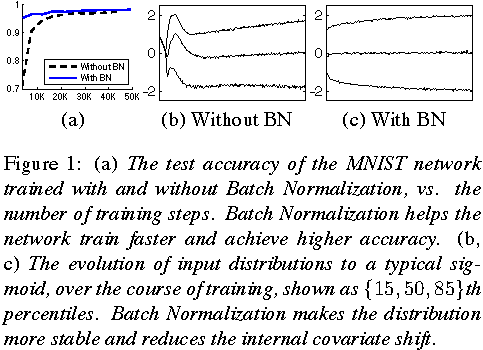
\includegraphics[width=0.9\textwidth]{BN_fig1.pdf}}
\end{frame}
%-------------------------------------------------------------%

\begin{frame}[fragile]{pause}\frametitle{Batch Normalization}
\center{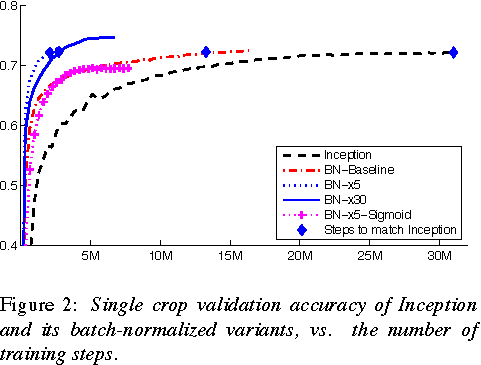
\includegraphics[width=0.9\textwidth]{BN_fig2.pdf}}
\end{frame}
%-------------------------------------------------------------%


%-------------------------------------------------------------%

% \begin{frame}[fragile]\frametitle{Variational Autoencoders (VAEs)}
% %\begin{center}
% 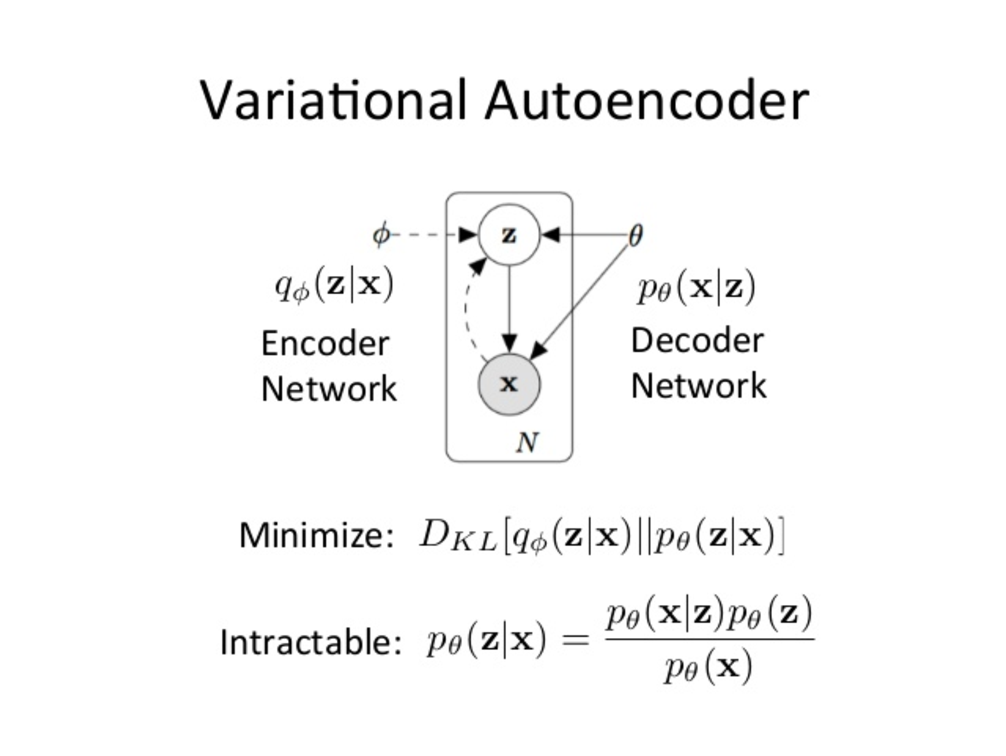
\includegraphics[width=10cm]{VAE.pdf} \footnote{Slide taken from \url{https://www.slideshare.net/ckmarkohchang/variational-autoencoder}}
% %\end{center}
% \end{frame}
% %-------------------------------------------------------------%

% \begin{frame}[fragile]{pause}\frametitle{Variational Autoencoder}
% \begin{itemize}
% \item In VAEs, data is generated by a directed graphical model $p(x|z)$. \pause
% \item The encoder is learning an approximation $q_{\phi}(z|x)$ to the posterior distribution $p_{\theta}(x|z)$, where $\phi$ and $\theta$ denote the parameters of the encoder and decoder, respectively. \pause
% \item The objective of the VAE has the following form $\mathcal{L} = D_{KL}(q_{\phi}(z|x) || p_{\theta}(z)) - \mathop{\mathbb{E}}_{q_{\phi}}(log  p_{\theta}(x|z))$
% \end{itemize}
% \end{frame}
% %-------------------------------------------------------------%